%%%%%%%%%%%%%%%%%%%%%%%%%%%%%%%%%%%%%%%%%
% University/School Laboratory Report
% LaTeX Template
% Version 3.1 (25/3/14)
%
% This template has been downloaded from:
% http://www.LaTeXTemplates.com
%
% Original author:
% Linux and Unix Users Group at Virginia Tech Wiki
% (https://vtluug.org/wiki/Example_LaTeX_chem_lab_report)
%
% License:
% CC BY-NC-SA 3.0 (http://creativecommons.org/licenses/by-nc-sa/3.0/)
%
%%%%%%%%%%%%%%%%%%%%%%%%%%%%%%%%%%%%%%%%%

%----------------------------------------------------------------------------------------
%	PACKAGES AND DOCUMENT CONFIGURATIONS
%----------------------------------------------------------------------------------------

\documentclass{article}

\usepackage[a4paper, total={6in, 9in}]{geometry}

\usepackage{siunitx} % Provides the \SI{}{} and \si{} command for typesetting SI units
\usepackage{graphicx} % Required for the inclusion of images
\usepackage{amsmath} % Required for some math elements
\usepackage[italian]{babel}
\usepackage{booktabs}% Better table spacing
\usepackage{subfig}
\usepackage{tikz}
\usepackage{pgfplots}
\pgfplotsset{compat=newest}
% axis style, ticks, etc
\pgfplotsset{every axis/.append style={
                    label style={font=\small},
                    tick label style={font=\footnotesize},
                    legend style={font=\scriptsize}
                    }}


\setlength\parindent{0pt} % Removes all indentation from paragraphs

\renewcommand{\labelenumi}{\alph{enumi}.} % Make numbering in the enumerate environment by letter rather than number (e.g. section 6)

%\usepackage{times} % Uncomment to use the Times New Roman font

\usepackage{tikz}
\usetikzlibrary{positioning}
\tikzset{%
  every neuron/.style={
    circle,
    draw,
    minimum size=1cm
  },
  neuron missing/.style={
    draw=none,
    scale=2,
    text height=0.333cm,
    execute at begin node=\color{black}$\vdots$
  },
}
\tikzstyle{line}=[draw]

% link and reference config
\usepackage{varioref}
\usepackage{hyperref}
\hypersetup{%
    pdfpagemode={UseOutlines},
    bookmarksopen,
    pdfstartview={FitH},
    colorlinks,
    linkcolor={black}, %COLORE DEI RIFERIMENTI AL TESTO
    citecolor={black}, %COLORE DEI RIFERIMENTI ALLE CITAZIONI
    urlcolor={black} %COLORI DEGLI URL
}

% compile tikz plots only once
\usetikzlibrary{trees}
\usetikzlibrary{external}
\usepgfplotslibrary{external}
\tikzexternalize[prefix=tex/]
\usepgfplotslibrary{units} % L A TEX and plain TEX
\usetikzlibrary{pgfplots.units} % L A TEX and plain TEX


%----------------------------------------------------------------------------------------
%	DOCUMENT INFORMATION
%----------------------------------------------------------------------------------------

\title{Rete neuronale per Ising e XY} % Title

\author{Martina \textsc{Crippa}, Pietro Francesco \textsc{Fontana}} % Author name

\date{\today} % Date for the report

\begin{document}

\maketitle % Insert the title, author and date

%\begin{center}
%\begin{tabular}{l r}
%Date Performed: & January 1, 2012 \\ % Date the experiment was performed
%Partners: & James Smith \\ % Partner names
%& Mary Smith \\
%Instructor: & Professor Smith % Instructor/supervisor
%\end{tabular}
%\end{center}

% If you wish to include an abstract, uncomment the lines below
% \begin{abstract}
% Abstract text
% \end{abstract}

%----------------------------------------------------------------------------------------
%	SECTION 1
%----------------------------------------------------------------------------------------

\section{Introduzione}
Nel campo della meccanica statistica un aspetto fondamentale è lo studio delle transizioni di fase, ovvero la trasformazione dello stato di un sistema al mutare di determinate variabili termodinamiche.
I sistemi considerati in questo lavoro, descritti dal modello di Ising e dal modello XY, transiscono al variare della temperatura e nel punto di passaggio questa viene detta temperatura di transizione.
In generale la transizione di fase è descritta da una funzione caratteristica del sistema, detta parametro d'ordine, ad esempio la magnetizzazione nel modello di Ising.
L'obiettivo del progetto è implementare e studiare una rete neuronale in grado di apprendere il parametro d'ordine per il modello di Ising e quindi classificare correttamente la fase di diverse configurazioni del sistema, individuando infine la temperatura di transizione.
Successivamente si è provato ad eseguire una procedura analoga nel caso del modello XY, un sistema che non presenta una transizione di fase descrivibile attraverso un parametro d'ordine, quindi dove la rete neuronale apprende altre caratteristiche del sistema per classificarne la fase.
Il lavoro prende spunto da diversi articoli pubblicati negli ultimi due anni che affrontano la stessa tematica \cite{carrasqu,melko,wessel}.

%----------------------------------------------------------------------------------------
%	SECTION 2
%----------------------------------------------------------------------------------------

\section{Sistemi fisici e simulazioni}
In questo lavoro sono stati simulati e studiati due sistemi classici della meccanica statistica su reticolo bidimensionale:  il modello di Ising e il modello XY.

\subsection{Modello di Ising}\label{sec:simIsing}
Il modello di Ising descrive il comportamento di spin su reticolo che assumono valori $\{+1;-1\}$ e interagiscono attraverso un'hamiltoniana la cui forma più semplice, utilizzata in questo lavoro, è
\begin{equation}
H=- \sum_{\langle i~j\rangle} \sigma_i\sigma_j
\end{equation}
dove le parentesi angolari indicano l'interazione a primi vicini fra gli spin $\sigma$.
Quindi viene assunto nullo il campo magnetico esterno e la costante di accoppiamento assume lo stesso valore fra tutti gli spin, pari a $1$.
Ad alte temperature il contributo entropico fa sì che il sistema si trovi in uno stato di disordine, ovvero nella fase paramagnetica, illustrata in figura \ref{fig:isingP}.
Abbassando la temperatura prevale l'interazione tra gli spin e al di sotto della temperatura di transizione questi tendono ad allinearsi, quindi il sistema transisce alla fase ferromagnetica, rappresentata in figura \ref{fig:isingF}.
Tale transizione di fase è detta del \emph{secondo ordine} ed è caratterizzata da un comportamento critico, per questo la temperatura di transizione viene anche detta temperatura critica.

\begin{figure}[ht]
\centering
\subfloat[Paramagnetico]{
\centering
\begin{tikzpicture}[> = stealth, scale=0.8]
\draw[gray,dashed,step=1.5cm] (-1,-1) grid +(5cm,5cm);
    \foreach \y in {0,1,2}
        \foreach \x in {0,1,2}
            \node[shape = rectangle, minimum width = 0.75cm, minimum height = 0.75cm] (dot_\y_\x) at (1.5*\x,1.5*\y){};

   \draw[ultra thick, ->]  (dot_0_0.south) -- (dot_0_0.north);
   \draw[ultra thick, <-]  (dot_1_1.south) -- (dot_1_1.north);
   \draw[ultra thick, <-]  (dot_2_1.south) -- (dot_2_1.north);
   \draw[ultra thick, ->]  (dot_1_2.south) -- (dot_1_2.north);
   \draw[ultra thick, <-]  (dot_2_2.south) -- (dot_2_2.north);
   \draw[ultra thick, <-]  (dot_0_2.south) -- (dot_0_2.north);
   \draw[ultra thick, ->]  (dot_2_0.south) -- (dot_2_0.north);
   \draw[ultra thick, ->]  (dot_0_1.south) -- (dot_0_1.north);
   \draw[ultra thick, <-]  (dot_1_0.south) -- (dot_1_0.north);
\end{tikzpicture}
\label{fig:isingP}
}
\subfloat[Ferromagnetico]{
\centering
\begin{tikzpicture}[> = stealth, scale=0.8]
\draw[gray,dashed,step=1.5cm] (-1,-1) grid +(5cm,5cm);
    \foreach \y in {0,1,2}
        \foreach \x in {0,1,2}
            {\node[shape = rectangle, minimum width = 0.75cm, minimum height = 0.75cm] (dot_\y_\x) at (1.5*\x,1.5*\y){};
            \draw[ultra thick, ->]  (dot_\y_\x.south) -- (dot_\y_\x.north);}
\end{tikzpicture}
\label{fig:isingF}
}
\caption{Ising 2D}
\end{figure}

Il parametro d'ordine che evidenzia la transizione di fase è la magnetizzazione per spin del sistema
\begin{equation}
m =\frac{1}{N} \sum_i \sigma_i
\end{equation}
Sono stati studiati sistemi con geometrie di reticolo differenti e conseguentemente aventi un numero di primi vicini (nn) e temperatura critica diversa, i valori sono riportati in tabella \ref{tab:ltI}.

\begin{table}[!ht]
\begin{center}
\begin{tabular}{rcccc}
\toprule
reticolo & nn & $T_c$ & $T_c$ approx $[$\si{K}$]$ & $T_{init}$ $[$\si{K}$]$\\
\midrule
honeycomb & $3$ & --- & $1.5187$ & $0.0$\\
quadrato & $4$ & $2/ \!\ln{(1+\sqrt{2})}$ & $2.2692$ & $1.0$\\
triangolare & $6$ & $4/\!\ln{3}$ & $3.6410 $ & $2.0$\\
\bottomrule
\end{tabular}
\end{center}
\caption{Reticoli studiati}
\label{tab:ltI}
\end{table}

La simulazione dei vari sistemi è stata effettuata con metodi Monte Carlo per $40$ diverse temperature distribuite simmetricamente attorno alla temperatura critica, specificando la temperatura iniziale $T_{init}$ riportata in tabella \ref{tab:ltI}.
Il sistema è stato inizializzato random a $T_{init}$, lasciandolo raggiungere l'equilibrio a temperatura fissata per poi passare alla temperatura successiva senza randomizzare nuovamente il sistema.
I modelli di Ising su reticolo quadrato e honeycomb sono stati simulati tramite l'algoritmo di Wolff \cite{wolff}, quindi eseguendo mosse a cluster, mentre il modello su reticolo triangolare è stato simulato con l'algoritmo di Metropolis, quindi ad ogni mossa viene provata l'inversione di un singolo spin.
Nelle simulazioni con l'algoritmo di Wolff il sistema di partenza è randomizzato, mentre nella simulazione con l'algoritmo di Metropolis il sistema di partenza è preso ordinato per facilitare il raggiungimento dell'equilibrio.
Le simulazioni sono state scritte in linguaggio C++, il generatore di numeri casuali utilizzato è il Mersenne Twister 19937.

\subsection{Modello XY}
Il modello XY descrive il comportamento di spin su reticolo in grado di ruotare assumendo valori nell'intervallo $[0,2\pi)$; gli spin interagiscono a primi vicini tramite l'hamiltoniana
\begin{equation}
H=-\sum_{\langle i~j\rangle} \cos(\theta_i-\theta_j)
\end{equation}
dove la costante si accoppiamento è stata fissata pari ad $1$ ed è stato posto nullo il campo magnetico esterno.
Nel modello XY,  secondo il teorema di Mermin-Wagner \cite{mermin}, non è prevista alcuna transizione di fase del secondo ordine.
Tuttavia presenta una transizione di fase \emph{topologica}, ovvero la transizione BKT \cite{kosterlitz}, che coinvolge la creazione di vortici e antivortici, configurazioni topologicamente stabili.
Appena sotto la temperatura di transizione si osserva la formazione di coppie vortice-antivortice mentre non è energeticamente conveniente la creazione di vortici e antivortici singoli, abbassando la temperatura la maggior parte degli spin tende ad orientarsi in modo parallelo.
Al di sopra della temperatura critica vince il contributo entropico e compaiono vortici e antivortici non accoppiati, gli spin in generale non sono più allineati tra loro.
Due configurazioni esemplari temperature diverse sono riportate in Figura \ref{fig:xy}.
Anche questo sistema è stato simulato tramite metodi Monte Carlo, utilizzando l'algoritmo di Wolff e seguendo una procedura analoga a quella utilizzata per il modello di Ising, i parametri sono riportati in tabella \ref{tab:ltXY}.

\begin{table}[ht]
\begin{center}
\begin{tabular}{rcccc}
\toprule
reticolo & nn & $T_t$ & $T_t$ approx $[$\si{K}$]$ & $T_{init}$ $[$\si{K}$]$\\
\midrule
quadrato & $4$ & --- & $0.893$ & $0.01$\\
\bottomrule
\end{tabular}
\end{center}
\caption{Reticoli studiati}
\label{tab:ltXY}
\end{table}
\begin{figure}[!ht]
\centering
\subfloat[Modello XY vicino alla temperatura critica]{
\centering
\begin{tikzpicture}[> = stealth, scale=0.7]
\draw[gray,dashed,step=1.5cm] (-1,-1) grid +(9.5cm,9.5cm);
    \foreach \y in {0,1,2,3,4,5}
        \foreach \x in {0,1,2,3,4,5}
            \node[shape = circle, minimum size = 0.6cm] (dot_\y_\x) at (1.5*\x,1.5*\y){};

    \draw[ultra thick,black, ->] (dot_0_0.2.79 r) -- (dot_0_0.pi r + 2.79 r);
    \draw[ultra thick,black, ->] (dot_0_1.3.38 r) -- (dot_0_1.pi r + 3.38 r);
    \draw[ultra thick,black, ->] (dot_0_2.3.50 r) -- (dot_0_2.pi r + 3.50 r);
    \draw[ultra thick,black, ->] (dot_0_3.2.99 r) -- (dot_0_3.pi r + 2.99 r);
    \draw[ultra thick,black, ->] (dot_0_4.2.51 r) -- (dot_0_4.pi r + 2.51 r);
    \draw[ultra thick,black, ->] (dot_0_5.2.63 r) -- (dot_0_5.pi r + 2.63 r);
    \draw[ultra thick,black, ->] (dot_1_0.3.46 r) -- (dot_1_0.pi r + 3.46 r);
    \draw[ultra thick,black, ->] (dot_1_1.2.45 r) -- (dot_1_1.pi r + 2.45 r);
    \draw[ultra thick,black, ->] (dot_1_2.2.67 r) -- (dot_1_2.pi r + 2.67 r);
    \draw[ultra thick,black, ->] (dot_1_3.2.63 r) -- (dot_1_3.pi r + 2.63 r);
    \draw[ultra thick,black, ->] (dot_1_4.2.07 r) -- (dot_1_4.pi r + 2.07 r);
    \draw[ultra thick,black, ->] (dot_1_5.1.50 r) -- (dot_1_5.pi r + 1.50 r);
    \draw[ultra thick,black, ->] (dot_2_0.2.29 r) -- (dot_2_0.pi r + 2.29 r);
    \draw[ultra thick,black, ->] (dot_2_1.3.38 r) -- (dot_2_1.pi r + 3.38 r);
    \draw[ultra thick,black, ->] (dot_2_2.2.82 r) -- (dot_2_2.pi r + 2.82 r);
    \draw[ultra thick,black, ->] (dot_2_3.1.92 r) -- (dot_2_3.pi r + 1.92 r);
    \draw[ultra thick,black, ->] (dot_2_4.3.19 r) -- (dot_2_4.pi r + 3.19 r);
    \draw[ultra thick,black, ->] (dot_2_5.5.22 r) -- (dot_2_5.pi r + 5.22 r);
    \draw[ultra thick,black, ->] (dot_3_0.3.24 r) -- (dot_3_0.pi r + 3.24 r);
    \draw[ultra thick,black, ->] (dot_3_1.2.81 r) -- (dot_3_1.pi r + 2.81 r);
    \draw[ultra thick,black, ->] (dot_3_2.3.68 r) -- (dot_3_2.pi r + 3.68 r);
    \draw[ultra thick,black, ->] (dot_3_3.3.74 r) -- (dot_3_3.pi r + 3.74 r);
    \draw[ultra thick,black, ->] (dot_3_4.2.65 r) -- (dot_3_4.pi r + 2.65 r);
    \draw[ultra thick,black, ->] (dot_3_5.0.78 r) -- (dot_3_5.pi r + 0.78 r);
    \draw[ultra thick,black, ->] (dot_4_0.2.24 r) -- (dot_4_0.pi r + 2.24 r);
    \draw[ultra thick,black, ->] (dot_4_1.3.17 r) -- (dot_4_1.pi r + 3.17 r);
    \draw[ultra thick,black, ->] (dot_4_2.2.86 r) -- (dot_4_2.pi r + 2.86 r);
    \draw[ultra thick,black, ->] (dot_4_3.2.93 r) -- (dot_4_3.pi r + 2.93 r);
    \draw[ultra thick,black, ->] (dot_4_4.3.16 r) -- (dot_4_4.pi r + 3.16 r);
    \draw[ultra thick,black, ->] (dot_4_5.3.12 r) -- (dot_4_5.pi r + 3.12 r);
    \draw[ultra thick,black, ->] (dot_5_0.2.79 r) -- (dot_5_0.pi r + 2.79 r);
    \draw[ultra thick,black, ->] (dot_5_1.2.89 r) -- (dot_5_1.pi r + 2.89 r);
    \draw[ultra thick,black, ->] (dot_5_2.3.30 r) -- (dot_5_2.pi r + 3.30 r);
    \draw[ultra thick,black, ->] (dot_5_3.2.76 r) -- (dot_5_3.pi r + 2.76 r);
    \draw[ultra thick,black, ->] (dot_5_4.2.53 r) -- (dot_5_4.pi r + 2.53 r);
    \draw[ultra thick,black, ->] (dot_5_5.2.91 r) -- (dot_5_5.pi r + 2.91 r);

    \node[draw, blue, ultra thick, shape = circle, minimum size = 0.8cm] at (1.5*4.5,1.5*2.5){};
    \node[draw, red, ultra thick, shape = circle, minimum size = 0.8cm] at (1.5*4.5,1.5*1.5){};
\end{tikzpicture}
}
\subfloat[Modello XY sopra la temperatura critica]{
\centering
\begin{tikzpicture}[> = stealth, scale=0.7]
\draw[gray,dashed,step=1.5cm] (-1,-1) grid +(9.5cm,9.5cm);
    \foreach \y in {0,1,2,3,4,5}
        \foreach \x in {0,1,2,3,4,5}
            \node[shape = circle, minimum size = 0.6cm] (dot_\y_\x) at (1.5*\x,1.5*\y){};

    \draw[ultra thick,black, ->] (dot_0_0.5.05 r) -- (dot_0_0.pi r + 5.05 r);
    \draw[ultra thick,black, ->] (dot_0_1.4.26 r) -- (dot_0_1.pi r + 4.26 r);
    \draw[ultra thick,black, ->] (dot_0_2.4.36 r) -- (dot_0_2.pi r + 4.36 r);
    \draw[ultra thick,black, ->] (dot_0_3.3.22 r) -- (dot_0_3.pi r + 3.22 r);
    \draw[ultra thick,black, ->] (dot_0_4.2.15 r) -- (dot_0_4.pi r + 2.15 r);
    \draw[ultra thick,black, ->] (dot_0_5.2.22 r) -- (dot_0_5.pi r + 2.22 r);
    \draw[ultra thick,black, ->] (dot_1_0.5.04 r) -- (dot_1_0.pi r + 5.04 r);
    \draw[ultra thick,black, ->] (dot_1_1.5.15 r) -- (dot_1_1.pi r + 5.15 r);
    \draw[ultra thick,black, ->] (dot_1_2.5.38 r) -- (dot_1_2.pi r + 5.38 r);
    \draw[ultra thick,black, ->] (dot_1_3.1.31 r) -- (dot_1_3.pi r + 1.31 r);
    \draw[ultra thick,black, ->] (dot_1_4.3.55 r) -- (dot_1_4.pi r + 3.55 r);
    \draw[ultra thick,black, ->] (dot_1_5.1.98 r) -- (dot_1_5.pi r + 1.98 r);
    \draw[ultra thick,black, ->] (dot_2_0.4.08 r) -- (dot_2_0.pi r + 4.08 r);
    \draw[ultra thick,black, ->] (dot_2_1.5.87 r) -- (dot_2_1.pi r + 5.87 r);
    \draw[ultra thick,black, ->] (dot_2_2.0.30 r) -- (dot_2_2.pi r + 0.30 r);
    \draw[ultra thick,black, ->] (dot_2_3.4.95 r) -- (dot_2_3.pi r + 4.95 r);
    \draw[ultra thick,black, ->] (dot_2_4.5.95 r) -- (dot_2_4.pi r + 5.95 r);
    \draw[ultra thick,black, ->] (dot_2_5.1.60 r) -- (dot_2_5.pi r + 1.60 r);
    \draw[ultra thick,black, ->] (dot_3_0.2.28 r) -- (dot_3_0.pi r + 2.28 r);
    \draw[ultra thick,black, ->] (dot_3_1.0.76 r) -- (dot_3_1.pi r + 0.76 r);
    \draw[ultra thick,black, ->] (dot_3_2.5.55 r) -- (dot_3_2.pi r + 5.55 r);
    \draw[ultra thick,black, ->] (dot_3_3.5.54 r) -- (dot_3_3.pi r + 5.54 r);
    \draw[ultra thick,black, ->] (dot_3_4.5.77 r) -- (dot_3_4.pi r + 5.77 r);
    \draw[ultra thick,black, ->] (dot_3_5.5.86 r) -- (dot_3_5.pi r + 5.86 r);
    \draw[ultra thick,black, ->] (dot_4_0.1.68 r) -- (dot_4_0.pi r + 1.68 r);
    \draw[ultra thick,black, ->] (dot_4_1.0.32 r) -- (dot_4_1.pi r + 0.32 r);
    \draw[ultra thick,black, ->] (dot_4_2.4.10 r) -- (dot_4_2.pi r + 4.10 r);
    \draw[ultra thick,black, ->] (dot_4_3.5.35 r) -- (dot_4_3.pi r + 5.35 r);
    \draw[ultra thick,black, ->] (dot_4_4.0.97 r) -- (dot_4_4.pi r + 0.97 r);
    \draw[ultra thick,black, ->] (dot_4_5.1.40 r) -- (dot_4_5.pi r + 1.40 r);
    \draw[ultra thick,black, ->] (dot_5_0.6.19 r) -- (dot_5_0.pi r + 6.19 r);
    \draw[ultra thick,black, ->] (dot_5_1.0.50 r) -- (dot_5_1.pi r + 0.50 r);
    \draw[ultra thick,black, ->] (dot_5_2.1.56 r) -- (dot_5_2.pi r + 1.56 r);
    \draw[ultra thick,black, ->] (dot_5_3.0.56 r) -- (dot_5_3.pi r + 0.56 r);
    \draw[ultra thick,black, ->] (dot_5_4.0.81 r) -- (dot_5_4.pi r + 0.81 r);
    \draw[ultra thick,black, ->] (dot_5_5.1.47 r) -- (dot_5_5.pi r + 1.47 r);

    \node[draw, blue, ultra thick, shape = circle, minimum size = 0.8cm] at (1.5*2.5,1.5*4.5){};
    \node[draw, blue, ultra thick, shape = circle, minimum size = 0.8cm] at (1.5*0.5,1.5*2.5){};
    \node[draw, red, ultra thick, shape = circle, minimum size = 0.8cm] at (1.5*4.5,1.5*1.5){};
    \node[draw, red, ultra thick, shape = circle, minimum size = 0.8cm] at (1.5*2.5,1.5*0.5){};
\end{tikzpicture}
}
\caption{Modello XY a due diverse temperature, i vortici sono indicati in blu, gli antivortici in rosso. Si può notare una chiara coppia vortice-antivortice nella figura di sinistra, mentre nella figura di destra non è presente alcuna coppia.}
\label{fig:xy}
\end{figure}

%----------------------------------------------------------------------------------------
%	SECTION 3
%----------------------------------------------------------------------------------------

\section{Metodi di apprendimento}
A partire dai sistemi fisici simulati, descritti nella sezione precedente, sono stati sviluppati diversi metodi di apprendimento con l'obiettivo di classificare automaticamente la fase in cui si trova il sistema.
I metodi utilizzati per l'apprendimento differiscono per i due modelli fisici analizzati, il modello di Ising e il modello XY, seguendo la stessa strada di altri lavori \cite{wessel}.

Le reti sono state implementate tramite Keras \cite{keras}, utilizzando Tensorflow \cite{tensorflow} come backend.

\subsection{Modello di Ising}

\begin{figure}[ht]
\centering
\resizebox{0.7\textwidth}{!}{
\begin{tikzpicture}[x=1.5cm, y=1.5cm, >=stealth, scale=1]

\foreach \m/\l [count=\y] in {1,2,missing,3}
  \node [every neuron/.try, neuron \m/.try] (input-\m) at (0,2.5-\y*1.35) {};

\foreach \m [count=\y] in {1,2,missing,3}
  \node [every neuron/.try, neuron \m/.try ] (hidden-\m) at (2,2.5-\y*1.35) {};

\node [circle,fill,inner sep=0.75pt] at (2.9166,2.5-1*1.35) {};
\node [circle,fill,inner sep=0.75pt] at (3.25,2.5-1*1.35) {};
\node [circle,fill,inner sep=0.75pt] at (3.5833,2.5-1*1.35) {};
\node [circle,fill,inner sep=0.75pt] at (2.9166,2.5-2*1.35) {};
\node [circle,fill,inner sep=0.75pt] at (3.25,2.5-2*1.35) {};
\node [circle,fill,inner sep=0.75pt] at (3.5833,2.5-2*1.35) {};
\node [circle,fill,inner sep=0.75pt] at (2.9166,2.5-4*1.35) {};
\node [circle,fill,inner sep=0.75pt] at (3.25,2.5-4*1.35) {};
\node [circle,fill,inner sep=0.75pt] at (3.5833,2.5-4*1.35) {};
\node [every neuron/.try, neuron missing/.try ] (hidden-missing) at (3.25,2.5-3*1.35) {};

\foreach \m [count=\y] in {1,2,missing,3}
  \node [every neuron/.try, neuron \m/.try ] (shidden-\m) at (4.5,2.5-\y*1.35) {};

\foreach \m [count=\y] in {1,2}
  \node [every neuron/.try, neuron \m/.try ] (output-\m) at (6.5,1-\y) {};

\foreach \l [count=\i] in {1,2,n}
  \draw [<-] (input-\i) -- ++(-1,0)
    node [above, midway] {$I_\l$};

\foreach \l [count=\i] in {1,2,m}
  \node [above] at (hidden-\i.north) {$H^1_\l$};

\foreach \l [count=\i] in {1,2,k}
  \node [above] at (shidden-\i.north) {$H^N_\l$};

\foreach \l [count=\i] in {1,2}
  \draw [->] (output-\i) -- ++(1,0)
    node [above, midway] {$O_\l$};

\foreach \i in {1,...,3}
  \foreach \j in {1,...,3}
    \draw [->] (input-\i) -- (hidden-\j);

\foreach \i in {1,...,3}
  \foreach \j in {1,...,2}
    \draw [->] (shidden-\i) -- (output-\j);

\node [align=center, above] at (0,2) {Layer \\ di Input};
\node [align=center, above] at (2,2) {Primo Layer \\ Nascosto};
\node [align=center, above] at (4.5,2) {N-esimo Layer \\ Nascosto};
\node [align=center, above] at (6.5,2) {Layer \\ di Output};

\end{tikzpicture}
}
\caption{Schema di una rete neuronale \emph{feed forward} a più layer nascosti \emph{fully connected}.}
\label{fig:ffn}
\end{figure}

Per classificare le configurazioni di un modello di Ising è stata utilizzata una rete neuronale \emph{feed forward} a uno o più layer nascosti, uno schema generico della rete è rappresentato in Figura \ref{fig:ffn}.
Al layer di input vengono fornite le configurazioni degli spin del sistema fisico nella forma di un vettore di elementi $\{+1;-1\}$, la dimensione di questo vettore dipende ovviamente dalla dimensione del reticolo di Ising utilizzato, nel caso del presente lavoro spazia da un minimo di 400 elementi (reticolo $20\times20$) ad un massimo di 8100 elementi (reticolo $90\times90$).
Le etichette con cui vengono classificate le configurazioni, e che vengono fornite per l'apprendimento, sono variabili binarie che indicano se il sistema si trova sopra o sotto la temperatura di transizione.

Si tratta di un problema di classificazione binaria, è quindi possibile utilizzare uno o due nodi nel layer di output, per una questione di comodità nell'analisi dei risultati fisici è stato utilizzato un layer di output a due nodi.
I nodi di output restituiscono la probabilità che la configurazione fisica sia in una fase ferromagnetica o in quella paramagnetica, le due probabilità sommano quindi a 1.

La rete viene sempre allenata su configurazioni del modello di Ising su reticolo quadrato classico, ossia con 4 primi vicini; se riesce ad apprendere correttamente la transizione di fase dovrebbe essere in grado di classificare adeguatamente anche le configurazioni dei modelli a lei sconosciuti, come Ising su reticolo triangolare e honeycomb.

\subsection{Modello XY}

\begin{figure}[ht]
 \centerline{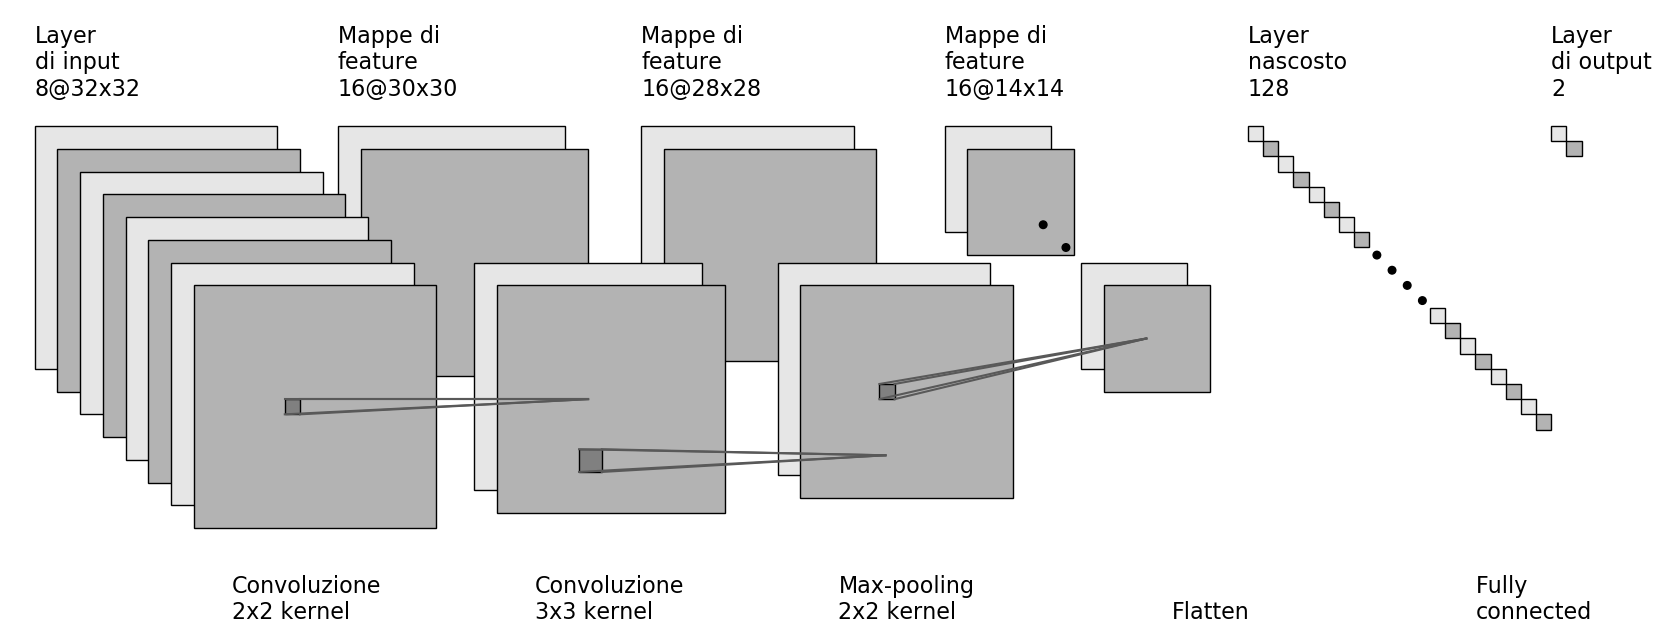
\includegraphics[scale=0.35]{cnn.png}}
 \caption{Schema di una rete convoluzionale effettivamente utilizzata per l'analisi di un sistema XY su reticolo $32\times32$, sono stati tralasciati i layer \emph{dropout}.}
 \label{fig:cnn}
\end{figure}

Il metodo migliore per classificare un modello XY risulta essere una rete convoluzionale \cite{melko}, uno schema di una rete di questo tipo effettivamente utilizzata in questo lavoro è rappresentato in Figura \ref{fig:cnn}.
Il layer di input può ricevere come argomento la semplice configurazione degli spin, quindi una matrice di valori reali nell'intervallo $[0,2\pi)$, oppure la configurazione espressa in vortici e antivortici, che appare come una matrice con valori $\{-1;0;+1\}$ che rappresentano rispettivamente la presenza di un antivortice, l'assenza di strutture e la presenza di un vortice.
Come nel caso di Ising le etichette indicano se la temperatura del sistema si trova sopra o sotto la temperatura di transizone e il layer di output ha due nodi, che rappresentano le probabilità complementari di essere in una delle due fasi.


%----------------------------------------------------------------------------------------
%	SECTION 4
%----------------------------------------------------------------------------------------

\section{Impostazione dell'apprendimento}

\begin{figure}[!ht]
\centering
\subfloat{
\begin{tikzpicture}
\begin{axis}[
    xlabel = {Epoche},
    ylabel = {Accuracy},
    grid = major,
    width=0.5\textwidth,
    height=0.5\textwidth,
    major grid style = {line width=.1pt, dashed, draw=gray!30},
    legend pos = south east,
]
\addplot+[mark=none, smooth, ultra thick]
    table[x=epoch, y=acc] {dati/training_histo_2};
\addlegendentry{Training accuracy}
\addplot+[mark=none, smooth, ultra thick]
    table[x=epoch, y=val_acc]{dati/training_histo_2};
\addlegendentry{Validation accuracy}
\end{axis}
\end{tikzpicture}
\label{fig:acc_histo}
}
\subfloat{
\begin{tikzpicture}
\begin{axis}[
    xlabel = {Epoche},
    ylabel = {Loss},
    grid = major,
    width=0.5\textwidth,
    height=0.5\textwidth,
    major grid style = {line width=.1pt, dashed, draw=gray!30},
    legend pos = north east,
]
\addplot+[mark=none, smooth, ultra thick]
    table[x=epoch, y=loss] {dati/training_histo_2};
\addlegendentry{Training loss}
\addplot+[mark=none, smooth, ultra thick]
    table[x=epoch, y=val_loss] {dati/training_histo_2};
\addlegendentry{Validation loss}
\end{axis}
\end{tikzpicture}
\label{fig:loss_histo}
}
\caption{Risultati dell'apprendimento di una rete \emph{feed forward} a singolo layer \emph{fully connected} da 100 neuroni. I dati utilizzati sono relativi ad un modello di Ising su reticolo quadrato di lato 30. Ogni punto è ottenuto come media della quantità considerata su 10 modelli allenati sullo stesso training set.}
\end{figure}

Il primo passo nel lavoro di creazione della rete è stato valutare se questa può apprendere efficacemente da un insieme di dati sufficientemente vasto.
Dopo aver generato circa \num{100000} dati per l'apprendimento questi sono stati divisi in \emph{training set} e \emph{validation set} in una percentuale rispettivamente dell'$80\%$ e del $20\%$.
Attraverso il \emph{validation set} è possibile stimare le performance della rete con l'avanzare del processo di apprendimento e capire se sta avvenendo un \emph{overfit}.

Lasciando apprendere la rete liberamente si è arrivati facilmente in situazioni in cui questa apprendeva caratteristiche chiaramente non generalizzabili ai dati esterni al \emph{training set}.
%TODO: figura curva bella bella di overfit, da fare
Per risolvere il problema sono stati introdotti dei regolarizzatori come L2, che limita la libertà di evoluzione dei pesi della rete, o come i layer \emph{dropout}, che disattivano alcuni nodi della rete in modo casuale; in generale questi metodi riescono ad impedire la costruzione di un modello perfetto per il \emph{training set} ed inevitabilmente meno generalizzabile.
Un altro utile strumento per la prevenzione dell'\emph{overfit} è l'\emph{early stop}, un metodo per interrompere in modo automatico l'apprendimento della rete una volta che le sue performance, valutate sul \emph{validation set}, siano sufficientemente stabili.
Applicando questi strumenti sono stati ottenuti ottimi risultati nell'apprendimento di sistemi di Ising e XY.
%TODO: figura curva bella bella senza overfit

\subsection{Statistica sui dati} \label{sec:stats}
Per ottenere in ogni analisi una stima solida delle variabili misurate, come la test accuracy, sono stati generati test set da \num{100000} elementi che vengono divisi in 10 insiemi più piccoli su cui ogni modello viene valutato.
Allo stesso modo, per tenere conto della componente stocastica presente nel processo di apprendimento della rete, sono stati generati 10 modelli su ciascun training set.
Questo procedimento genera quindi 10 misure per ciascuno dei 10 modelli, per un totale di 100 misure, da cui viene estratta la media e l'errore, come deviazione standard della media.
Questo sarà lo standard utilizzato in tutte le analisi successive.

%----------------------------------------------------------------------------------------
%	SECTION 5
%----------------------------------------------------------------------------------------

\section{Modello di Ising: risultati e conclusioni}

\subsection{Valutazione dei parametri della rete}
Per meglio valutare il contributo dei diversi parametri della rete sono stati generati più modelli, eseguendo la fase di apprendimento sullo stesso training set e variando di volta in volta alcune caratteristiche quali il numero di neuroni in un layer o il numero di layer.

\subsubsection{Diverso numero di neuroni}
La prima analisi è stata effettuata allenando diverse reti a singolo layer nascosto con numero di neuroni variabile, i valori esplorati sono: 3, 10, 50, 100, 200 e 1000.
L'analisi è stata limitata a modelli di Ising su reticoli di lato 30, 50 e 80.
Nel grafico in figura \ref{fig:NN} sono riportati i valori di test accuracy al variare del numero di neuroni, rappresentati in scala logaritmica.

Si osserva che per il reticolo di lato 30 una rete a 10 neuroni è sufficiente per classificare in maniera adeguata la fase del sistema, raggiungendo una test accuracy circa del $98\%$.
Per reticoli di maggiori dimensioni sono necessari almeno 50 neuroni per raggiungre livelli di test accuracy superiori al $90\%$.
Per tutte le dimensioni considerate aumentando il numero di neuroni a 1000 si osserva un crollo nelle performance per i reticoli honeycomb e quadrato, mentre per il reticolo triangolare la rete continua a classificare in modo soddisfacente.
Per limiti computazionali non sono state realizzate reti con un numero di neuroni superiore, quindi non è stato possibile chiarire l'andamento complessivo per il reticolo triangolare.
Si osserva che una differenza tra la configurazione su reticolo triangolare e gli altri due sistemi, oltre alla geometria del reticolo, è l'algoritmo utilizzato per la simulazione del sistema, come riportato in sezione \ref{sec:simIsing}.
%TODO approfondire la cosa

\begin{figure}[!ht]
\centering
\subfloat{
\begin{tikzpicture}
\begin{axis}[
    title=Honeycomb,
    xmode=log,
    xlabel = {Numero di neuroni},
    ylabel = {Test accuracy},
    grid = major,
    width=0.35\textwidth,
    height=0.44\textwidth,
    major grid style = {line width=.1pt, dashed, draw=gray!30},
    legend pos = south east,
]
\addplot+[line, mark=*, error bars/.cd, y dir = both, y explicit, error mark=none, error bar style=thick]
    table[x=neurons, y=accuracy, y error=stdev] {dati/neurons_number/neurons_number_900_hc};
\addlegendentry{L30}
\addplot+[line, mark=square*, error bars/.cd, y dir = both, y explicit, error mark=none, error bar style=thick]
    table[x=neurons, y=accuracy, y error=stdev] {dati/neurons_number/neurons_number_2500_hc};
\addlegendentry{L50}
\addplot+[line, mark=triangle*, error bars/.cd, y dir = both, y explicit, error mark=none, error bar style=thick]
    table[x=neurons, y=accuracy, y error=stdev] {dati/neurons_number/neurons_number_6400_hc};
\addlegendentry{L80}
\end{axis}
\end{tikzpicture}
}
\subfloat{
\begin{tikzpicture}
\begin{axis}[
    title=Quadrato,
    xmode=log,
    xlabel = {Numero di neuroni},
    grid = major,
    width=0.35\textwidth,
    height=0.44\textwidth,
    major grid style = {line width=.1pt, dashed, draw=gray!30},
    legend pos = south east,
]
\addplot+[line, mark=*, error bars/.cd, y dir = both, y explicit, error mark=none, error bar style=thick]
    table[x=neurons, y=accuracy, y error=stdev] {dati/neurons_number/neurons_number_900_sq};
\addlegendentry{L30}
\addplot+[line, mark=square*, error bars/.cd, y dir = both, y explicit, error mark=none, error bar style=thick]
    table[x=neurons, y=accuracy, y error=stdev] {dati/neurons_number/neurons_number_2500_sq};
\addlegendentry{L50}
\addplot+[line, mark=triangle*, error bars/.cd, y dir = both, y explicit, error mark=none, error bar style=thick]
    table[x=neurons, y=accuracy, y error=stdev] {dati/neurons_number/neurons_number_6400_sq};
\addlegendentry{L80}
\end{axis}
\end{tikzpicture}
}
\subfloat{
\begin{tikzpicture}
\begin{axis}[
    title=Triangolare,
    xmode=log,
    xlabel = {Numero di neuroni},
    grid = major,
    width=0.35\textwidth,
    height=0.44\textwidth,
    major grid style = {line width=.1pt, dashed, draw=gray!30},
    legend pos = south east,
]
\addplot+[line, mark=*, error bars/.cd, y dir = both, y explicit, error mark=none, error bar style=thick]
    table[x=neurons, y=accuracy, y error=stdev] {dati/neurons_number/neurons_number_900_tr};
\addlegendentry{L30}
\addplot+[line, mark=square*, error bars/.cd, y dir = both, y explicit, error mark=none, error bar style=thick]
    table[x=neurons, y=accuracy, y error=stdev] {dati/neurons_number/neurons_number_2500_tr};
\addlegendentry{L50}
\addplot+[line, mark=triangle*, error bars/.cd, y dir = both, y explicit, error mark=none, error bar style=thick]
    table[x=neurons, y=accuracy, y error=stdev] {dati/neurons_number/neurons_number_6400_tr};
\addlegendentry{L80}
\end{axis}
\end{tikzpicture}
}
\caption{Performance della rete feed forward a singolo layer fully connected sul modello di Ising.}
\label{fig:NN}
\end{figure}

\subsubsection{Diverso numero di layer}

\begin{figure}[!ht]
\centering
\subfloat{
\begin{tikzpicture}
\begin{axis}[
    xlabel = {Numero di neuroni},
    ylabel = {\# parametri / \# training data},
    grid = major,
    width=0.5\textwidth,
    height=0.5\textwidth,
    major grid style = {line width=.1pt, dashed, draw=gray!30},
    legend pos = north west,
]
\addplot+[line, thick, mark=*]
    table[x=neurons, y expr={\thisrow{param}/\thisrow{datatr}}] {dati/neurons_number/neurons_param_900};
\addlegendentry{L30}
\addplot+[line, thick, mark=square*]
    table[x=neurons, y expr={\thisrow{param}/\thisrow{datatr}}] {dati/neurons_number/neurons_param_2500};
\addlegendentry{L50}
\addplot+[line, thick, mark=triangle*]
    table[x=neurons, y expr={\thisrow{param}/\thisrow{datatr}}] {dati/neurons_number/neurons_param_6400};
\addlegendentry{L80}
\end{axis}
\end{tikzpicture}
}
\subfloat{
\begin{tikzpicture}
\begin{axis}[
    xlabel = {Numero di layer nascosti},
    ymax=1.5,
    grid = major,
    width=0.5\textwidth,
    height=0.5\textwidth,
    major grid style = {line width=.1pt, dashed, draw=gray!30},
    legend pos = north west,
]
\addplot+[line, thick, mark=*]
    table[x=layers, y expr={\thisrow{param}/\thisrow{datatr}}] {dati/layers_number/layers_param_900};
\addlegendentry{L30}
\addplot+[line, thick, mark=square*]
    table[x=layers, y expr={\thisrow{param}/\thisrow{datatr}}] {dati/layers_number/layers_param_2500};
\addlegendentry{L50}
\addplot+[line, thick, mark=triangle*]
    table[x=layers, y expr={\thisrow{param}/\thisrow{datatr}}] {dati/layers_number/layers_param_6400};
\addlegendentry{L80}
\end{axis}
\end{tikzpicture}
}
\caption{Rapporto tra il numero di parametri della rete e il numero di elementi del training set utilizzato per l'apprendimento.}
\label{fig:par}
\end{figure}

Il primo grafico riportato in figura \ref{fig:par} presenta l'andamento del numero di parametri normalizzato sul numero di training data rispetto al numero di neuroni per reti a un layer nascosto.
Come si può notare il numero di parametri segue un andamento lineare e cresce velocemente.
Diversamente, nel secondo grafico in figura \ref{fig:par} si osserva che aumentando il numero di layer il numero di parametri cresce sempre linearmente ma in maniera molto meno marcata, la crescita è rappresentata rispetto al numero di layer nascosti che è proporzionale al numero totale di neuroni.

Un buon equilibrio tra il numero di parametri da apprendere ed il numero di dati utilizzati per l'apprendimento porta tendenzialmente ad ottenere migliori risultati.
%TODO verificare
Perciò è stata effettuata una seconda analisi cercando di mantenere un numero di parametri rispetto al numero di dati costante per ciascun reticolo, allenando reti a più layer nascosti, pari a  1, 2, 3, 5 e 10 con ciascun layer popolato da 10 neuroni.
I risultati, riportati nei grafici di \ref{fig:LN}, mostrano che si ottiene un valore ottimale di test accuracy per tutte le tipologie di reticolo classificando con reti a 2 layer. Aggiungendo un layer le performance si abbassano notevolmente, mentre per i reticoli di lato 30 si ottengono buoni risultati anche per reti aventi  un singolo layer.
Inoltre dai risultati di questa analisi si può osservare come le performance sul modello di Ising con reticolo triangolare siano consistenti con quelle degli altri modelli, al contrario di quanto riportato nella sezione precedente.
%TODO: da approfondire

\begin{figure}[!ht]
\centering
\subfloat{
\begin{tikzpicture}
\begin{axis}[
    title=Honeycomb,
    xlabel = {Numero di layer nascosti},
    ylabel = {Test accuracy},
    grid = major,
    width=0.35\textwidth,
    height=0.44\textwidth,
    major grid style = {line width=.1pt, dashed, draw=gray!30},
    legend pos = north east,
]
\addplot+[line, mark=*, error bars/.cd, y dir = both, y explicit, error mark=none, error bar style=thick]
    table[x=layers, y=accuracy, y error=stdev] {dati/layers_number/layers_number_900_hc};
\addlegendentry{L30}
\addplot+[line, mark=square*, error bars/.cd, y dir = both, y explicit, error mark=none, error bar style=thick]
    table[x=layers, y=accuracy, y error=stdev] {dati/layers_number/layers_number_2500_hc};
\addlegendentry{L50}
\addplot+[line, mark=triangle*, error bars/.cd, y dir = both, y explicit, error mark=none, error bar style=thick]
    table[x=layers, y=accuracy, y error=stdev] {dati/layers_number/layers_number_6400_hc};
\addlegendentry{L80}
\end{axis}
\end{tikzpicture}
}
\subfloat{
\begin{tikzpicture}
\begin{axis}[
    title=Quadrato,
    xlabel = {Numero di layer nascosti},
    grid = major,
    width=0.35\textwidth,
    height=0.44\textwidth,
    major grid style = {line width=.1pt, dashed, draw=gray!30},
    legend pos = north east,
]
\addplot+[line, mark=*, error bars/.cd, y dir = both, y explicit, error mark=none, error bar style=thick]
    table[x=layers, y=accuracy, y error=stdev] {dati/layers_number/layers_number_900_sq};
\addlegendentry{L30}
\addplot+[line, mark=square*, error bars/.cd, y dir = both, y explicit, error mark=none, error bar style=thick]
    table[x=layers, y=accuracy, y error=stdev] {dati/layers_number/layers_number_2500_sq};
\addlegendentry{L50}
\addplot+[line, mark=triangle*, error bars/.cd, y dir = both, y explicit, error mark=none, error bar style=thick]
    table[x=layers, y=accuracy, y error=stdev] {dati/layers_number/layers_number_6400_sq};
\addlegendentry{L80}
\end{axis}
\end{tikzpicture}
}
\subfloat{
\begin{tikzpicture}
\begin{axis}[
    title=Triangolare,
    xlabel = {Numero di layer nascosti},
    grid = major,
    width=0.35\textwidth,
    height=0.44\textwidth,
    major grid style = {line width=.1pt, dashed, draw=gray!30},
    legend pos = north east,
]
\addplot+[line, mark=*, error bars/.cd, y dir = both, y explicit, error mark=none, error bar style=thick]
    table[x=layers, y=accuracy, y error=stdev] {dati/layers_number/layers_number_900_tr};
\addlegendentry{L30}
\addplot+[line, mark=square*, error bars/.cd, y dir = both, y explicit, error mark=none, error bar style=thick]
    table[x=layers, y=accuracy, y error=stdev] {dati/layers_number/layers_number_2500_tr};
\addlegendentry{L50}
\addplot+[line, mark=triangle*, error bars/.cd, y dir = both, y explicit, error mark=none, error bar style=thick]
    table[x=layers, y=accuracy, y error=stdev] {dati/layers_number/layers_number_6400_tr};
\addlegendentry{L80}
\end{axis}
\end{tikzpicture}
}
\caption{Performance della rete feed forward a layer multipli fully connected da dieci neuroni ciascuno sul modello di Ising.}
\label{fig:LN}
\end{figure}

Tuttavia confrontando i valori in tabella \ref{tab:NNLN} si può notare come l'apprendimento sul modello di Ising non sembri trarre vantaggio dall'utilizzo di reti a più layer.

\begin{table}[ht]
\begin{center}
\begin{tabular}{lcc}
\toprule
L & 1x100 test accuracy & 2x10 test accuracy\\
\midrule
30 & \num{0.981 \pm 0.004} & \num{0.979 \pm 0.004} \\
50 & \num{0.973 \pm 0.006} & \num{0.988 \pm 0.003} \\
80 & \num{0.994 \pm 0.002} & \num{0.993 \pm 0.002} \\
\bottomrule
\end{tabular}
\end{center}
\caption{Test accuracy valutata su una rete a singolo layer da 100 neuroni e su una rete a 2 layer da 10 neuroni ciascuno. I valori sono la media sulle tre diverse tipologie di reticolo per ciascuna dimensione, l'errore è stimato come deviazione standard della media.}
\label{tab:NNLN}
\end{table}

\subsubsection{Due layer e diverso numero di neuroni}
I risltati delle analisi descritte nei capitoli precedenti, riportati in tabella \ref{tab:NNLN}, mostrano che per tutti modelli considerati si ottengono valori di test accuracy massimi per reti a singolo layer con 100 neuroni e per reti a 2 layer con 10 neuroni per layer.

Prendendo spunto da questi risultati sono stati generati modelli di rete a 2 layer, con un numero totale di neuroni pari a 100, variando il numero di neuroni dei diversi layer.
 Si è iniziato allenando una rete a 30 e 70 neuroni per i due rispettivi layer, quindi fornendo ad entrambi i layer un numero consistente di neuroni.
Come si può osservare dai risultati riportati in tabella \ref{tab:2LN30-70}, questi sono compatibili entro l'errore con quelli riportati in tabella \ref{tab:NNLN}, a parte la test accuracy per la rete 1x100 sul reticolo L50 che si discosta di circa $2\sigma$ dagli altri valori.
Inoltre, anche invertendo i layer da 30 e 70 neuroni si ottengono valori di test accuracy uguali entro l'errore.

\begin{table}[ht]
\begin{center}
\begin{tabular}{lcc}
\toprule
L & 1x70+1x30 test accuracy & 1x30+1x70 test accuracy\\
\midrule
30 & \num{0.979 \pm 0.004} & \num{0.978 \pm 0.005} \\
50 & \num{0.988 \pm 0.003} & \num{0.988 \pm 0.003} \\
80 & \num{0.993 \pm 0.002} & \num{0.993 \pm 0.002} \\
\bottomrule
\end{tabular}
\end{center}
\caption{Test accuracy valutata su una rete a 2 layer da 70 e 30 neuroni e su una rete a 2 layer da 30 e 70 neuroni. I valori sono la media sulle tre diverse tipologie di reticolo per ciascuna dimensione, l'errore è stimato come deviazione standard della media.}
\label{tab:2LN30-70}
\end{table}

Quindi, nel caso di una rete a due layer entrambi con un numero consistente di neuroni, l'inversione dei layer non sembrerebbe modificare le sue capacità di apprendimento.
Si procede allenando una rete sempre a due layer, con un numero di neuroni per layer meno equilibrato: 95 e 5.

\begin{table}[ht]
\begin{center}
\begin{tabular}{lcc}
\toprule
L & 1x95+1x5 test accuracy & 1x5+1x95 test accuracy\\
\midrule
30 & \num{0.979 \pm 0.004} & \num{0.978 \pm 0.004} \\
50 & \num{0.988 \pm 0.003} & \num{0.987 \pm 0.003} \\
80 & \num{0.0 \pm 0.0} & \num{0.0 \pm 0.0} \\
\bottomrule
\end{tabular}
\end{center}
\caption{Test accuracy valutata su una rete a 2 layer da 95 e 5 neuroni e su una rete a 2 layer da 5 e 95 neuroni. I valori sono la media sulle tre diverse tipologie di reticolo per ciascuna dimensione, l'errore è stimato come deviazione standard della media.}
\label{tab:2LN5-95}
\end{table}

Anche in questo caso si osserva che i risultati riportati in tabella \ref{tab:2LN5-95} sono assolutamente compatibili con i risultati in tabella \ref{tab:2LN30-70}, quindi la rete non risulta essere sensibile all'inversione di layer, al contrario di quanto ci si sarebbe potuto aspettare: infatti l'inversione di layer porta a una diminuzione del numero di parametri per numero di dati, come riportato in tabella \ref{tab:LNparam}.

\begin{table}[ht]
\begin{center}
\begin{tabular}{clll}
\toprule
Rete & L30 & L50 & L80\\
\midrule
1x70+1x30 & \num{0.81} & \num{2.22} & \num{5.62}\\
1x30+1x70 & \num{0.36} & \num{0.97} & \num{2.43}\\
\midrule
1x95+1x5 & \num{1.07} & \num{2.98} &\\
1x5+1x95 & \num{0.07} & \num{0.17} & \\
\bottomrule
\end{tabular}
\end{center}
\caption{Numero di parametri normalizzato sul numero di dati del training set}
\label{tab:LNparam}
\end{table}

\subsubsection{Diversa funzione di attivazione}
\subsection{Stima delle tempistiche di training}
\subsection{Stima della temperatura critica}
Attraverso l'utilizzo delle reti neuronali, è stato possibile stimare la temperatura critica $T_c$ del modello di Ising, riportata nell'introduzione.
Tale valore teorico è esatto per sistemi su reticolo di lato infinito; per sistemi di lato finito la temperatura critica presenta una correzione che aumenta al diminuire della dimensione del reticolo.
Per stimare il valore teorico è stato effettuato il calcolo della temperatura critica su diversi reticoli al variare della lato del reticolo (in numero di spin) da 20 a 90, con passo 10, andando poi ad interpolare i risultati e ottenendo il valore per $L\rightarrow \infty$.
%TODO provare a cercare la legge
La rete è stata allenata su set di almeno \num{100000} configurazioni (prendendo un sottoinsieme di configurazioni pari al $20\%$ del training set per la validazione) a reticolo quadrato, e testata su set di \num{100000} a reticolo sia triangolare che honeycomb.
Ciascun valore di temperatura riportato è dato dalla media di 100 temperature, i cui valori sono classificati da 10 diverse reti su 10 diversi test set, come spiegato nella sezione \ref{sec:stats}.
Le reti utilizzate per questo scopo sono state scelte appositamente, tra quelle con test accuracy alta e test loss bassa.
I parametri della rete sono riportati in tabella \ref{tab:ffnnpar}

\begin{table}[ht]
\begin{center}
\begin{tabular}{ll}
\toprule
Layer: & 1\\
Neuroni: & 100 \\
Batch size: & 100\\
Pesi w e b iniziali: & Random\\
Fz. attivazione: & Sigmoidale\\
Earlystop: & validation acc \\
Regolarizzazione: & L2 0.01\\
Ottimizzazione: & Adam 0.0001 \\
\bottomrule
\end{tabular}
\end{center}
\caption{Parametri}
\label{tab:ffnnpar}
\end{table}

Nei grafici in figura \ref{fig:Tlimit} sono riportate le medie delle temperature $T_L$ al variare del lato del reticolo, con le relative barre d'errore date dalla deviazione standard della media.
Inoltre è riportato il valore teorico della temperatura di transizione $T_c$ e la retta che interpola tali temperature.

\begin{figure}[ht]
\centering
\subfloat{
\begin{tikzpicture}
\begin{axis}[
    title={Honeycomb},
    ylabel={$T$ [\si{K}]},
    xlabel={$L^{-1}$  [$\si{nspin}^{-1}$]},
    width=0.33\textwidth,
    height=0.44\textwidth,
    xmin=0.0,
    xmax=0.06,
    minor y tick num=1,
    ytick={1.51,1.52,1.53,1.54},
    grid=both,
    minor grid style={line width=.1pt, dashed, draw=gray!30},
    major grid style={line width=.1pt, dashed, draw=gray!30},
    legend pos=north west
]
\addplot+[mark=none, red, thick] coordinates {(0.0,1.5187) (0.06,1.5187)};
\addlegendentry{$T_c$}
\addplot[only marks, blue, mark=*, error bars/.cd, y dir = both, y explicit, error mark=none, error bar style=thick]
     table [x expr={1/\thisrow{size}}, y=temp, y error=temp_e] {dati/temperature_hc};
\addlegendentry{$T_L$}
\addplot+[mark=none, green!70!black, thick, domain=0.01:0.055, samples=101]{0.2939*x + 1.5151};
\end{axis}
\end{tikzpicture}
}
\subfloat{
\begin{tikzpicture}
\begin{axis}[
    title={Quadrato},
    xlabel = {$L^{-1}$  [$\si{nspin}^{-1}$]},
    width=0.33\textwidth,
    height=0.44\textwidth,
    xmin=0.0,
    xmax=0.06,
    minor y tick num=1,
    ytick={2.25,2.26,2.27,2.28,2.29,2.30},
    grid=both,
    minor grid style={line width=.1pt, dashed, draw=gray!30},
    major grid style={line width=.1pt, dashed, draw=gray!30},
    legend pos=north west
]
\addplot+[mark=none, red, thick] coordinates {(0.0,2.2692) (0.06,2.2692)};
\addlegendentry{$T_c$}
\addplot[only marks, blue, mark=*, error bars/.cd, y dir = both, y explicit, error mark=none, error bar style=thick]
     table [x expr={1/\thisrow{size}}, y=temp, y error=temp_e] {dati/temperature_sq};
\addlegendentry{$T_L$}
\addplot+[mark=none, green!70!black, thick, domain=0.01:0.055, samples=101]{0.4167*x + 2.2653};
\end{axis}
\end{tikzpicture}
}
\subfloat{
\begin{tikzpicture}
\begin{axis}[
    title={Triangolare},
    xlabel = {$L^{-1}$  [$\si{nspin}^{-1}$]},
    width=0.33\textwidth,
    height=0.44\textwidth,
    xmin=0.0,
    xmax=0.06,
    minor y tick num=1,
    ytick={3.62,3.63,3.64,3.65,3.66},
    grid=both,
    minor grid style={line width=.1pt, dashed, draw=gray!30},
    major grid style={line width=.1pt, dashed, draw=gray!30},
    legend pos=north west
]
\addplot+[mark=none, red, thick] coordinates {(0.0,3.6410) (0.06,3.6410)};
\addlegendentry{$T_c$}
\addplot[only marks, blue, mark=*, error bars/.cd, y dir = both, y explicit, error mark=none, error bar style=thick]
     table [x expr={1/\thisrow{size}}, y=temp, y error=temp_e] {dati/temperature_tr};
\addlegendentry{$T_L$}
\addplot+[mark=none, green!70!black, thick, domain=0.01:0.055, samples=101]{0.3994*x + 3.6348};
\end{axis}
\end{tikzpicture}
}
\caption{Interpolazione temperatura}
\label{fig:Tlimit}
\end{figure}

In tabella \ref{tab:Tising} sono riportati i valori estratti per la temperatura di transizione, il valore riportato è il termine costante della retta estratta tramite un fit eseguito con il metodo dei minimi quadrati.

\begin{table}[ht]
\begin{center}
\begin{tabular}{rcc}
\toprule
Reticolo & T estratta & T teorica \\
\midrule
honeycomb & \num{1.52 \pm 0.04} & \num{1.519} \\
quadrato & \num{2.27 \pm 0.07} & \num{2.269} \\
triangolare & \num{3.63 \pm 0.16} & \num{3.641} \\
\bottomrule
\end{tabular}
\end{center}
\caption{Valori ottenuti tramite il fit per la temperatura di transizione. I valori teorici esatti sono riportati in tabella \ref{tab:ltI}.}
\label{tab:Tising}
\end{table}

%----------------------------------------------------------------------------------------
%	LAST SECTION
%----------------------------------------------------------------------------------------

\section{Modello XY: risultati e conclusioni}
\subsection{Valutazione dei parametri della rete}
Analogamente a quanto svolto per il modello di Ising si è provato a variare qualche parametro della rete convoluzionale utilizzata per il modello XY.
%----------------------------------------------------------------------------------------
%	APPENDICES
%----------------------------------------------------------------------------------------

\appendix

\section{Dati tabulati}


%----------------------------------------------------------------------------------------
%	BIBLIOGRAPHY
%----------------------------------------------------------------------------------------

\bibliographystyle{ieeetr}

\bibliography{relazione}

%----------------------------------------------------------------------------------------


\end{document}
